%%%%%%%%%%%%%%%%%%%%%%%%%%%%%%%%%%%%%%%%%
% Beamer Presentation
% LaTeX Template
% Version 1.0 (10/11/12)
%
% This template has been downloaded from:
% http://www.LaTeXTemplates.com
%
% License:
% CC BY-NC-SA 3.0 (http://creativecommons.org/licenses/by-nc-sa/3.0/)
%
%%%%%%%%%%%%%%%%%%%%%%%%%%%%%%%%%%%%%%%%%

%----------------------------------------------------------------------------------------
%    PACKAGES AND THEMES
%----------------------------------------------------------------------------------------

\documentclass[usenames,dvipsnames]{beamer}
\usepackage{animate}
\usepackage{float}
\usepackage{bm}
\usepackage{mathtools}
\usepackage{extarrows}
\usepackage[utf8]{inputenc}
\usepackage[english]{babel}
\usepackage{minted}
\newcommand{\ChoL}{\mathsf{L}}
\newcommand{\bx}{\mathbf{x}}
\newcommand{\ii}{\mathrm{i}}
\newcommand{\bxi}{\bm{\xi}}
\newcommand{\bmu}{\bm{\mu}}
\newcommand{\bb}{\mathbf{b}}
\newcommand{\bA}{\mathbf{A}}
\newcommand{\bJ}{\mathbf{J}}
\newcommand{\bB}{\mathbf{B}}
\newcommand{\bM}{\mathbf{M}}

\newcommand{\by}{\mathbf{y}}
\newcommand{\bw}{\mathbf{w}}

\newcommand{\bX}{\mathbf{X}}
\newcommand{\bY}{\mathbf{Y}}
\newcommand{\bs}{\mathbf{s}}
\newcommand{\sign}{\mathrm{sign}}
\newcommand{\bt}[0]{\bm{\theta}}
\newcommand{\bc}{\mathbf{c}}
\newcommand{\bzero}{\mathbf{0}}
\renewcommand{\bf}{\mathbf{f}}
\newcommand{\bu}{\mathbf{u}}
\newcommand{\bv}[0]{\mathbf{v}}

\mode<presentation> {

% The Beamer class comes with a number of default slide themes
% which change the colors and layouts of slides. Below this is a list
% of all the themes, uncomment each in turn to see what they look like.

%\usetheme{default}
%\usetheme{AnnArbor}
%\usetheme{Antibes}
%\usetheme{Bergen}
%\usetheme{Berkeley}
%\usetheme{Berlin}
%\usetheme{Boadilla}
%\usetheme{CambridgeUS}
%\usetheme{Copenhagen}
%\usetheme{Darmstadt}
%\usetheme{Dresden}
%\usetheme{Frankfurt}
%\usetheme{Goettingen}
%\usetheme{Hannover}
%\usetheme{Ilmenau}
%\usetheme{JuanLesPins}
%\usetheme{Luebeck}
\usetheme{Madrid}
%\usetheme{Malmoe}
%\usetheme{Marburg}
%\usetheme{Montpellier}
%\usetheme{PaloAlto}
%\usetheme{Pittsburgh}
%\usetheme{Rochester}
%\usetheme{Singapore}
%\usetheme{Szeged}
%\usetheme{Warsaw}


% As well as themes, the Beamer class has a number of color themes
% for any slide theme. Uncomment each of these in turn to see how it
% changes the colors of your current slide theme.

%\usecolortheme{albatross}
\usecolortheme{beaver}
%\usecolortheme{beetle}
%\usecolortheme{crane}
%\usecolortheme{dolphin}
%\usecolortheme{dove}
%\usecolortheme{fly}
%\usecolortheme{lily}
%\usecolortheme{orchid}
%\usecolortheme{rose}
%\usecolortheme{seagull}
%\usecolortheme{seahorse}
%\usecolortheme{whale}
%\usecolortheme{wolverine}

%\setbeamertemplate{footline} % To remove the footer line in all slides uncomment this line
%\setbeamertemplate{footline}[page number] % To replace the footer line in all slides with a simple slide count uncomment this line

%\setbeamertemplate{navigation symbols}{} % To remove the navigation symbols from the bottom of all slides uncomment this line
}
\usepackage{booktabs}
\usepackage{makecell}
\usepackage{soul}
\newcommand{\red}[1]{\textcolor{red}{#1}}
%
%\usepackage{graphicx} % Allows including images
%\usepackage{booktabs} % Allows the use of \toprule, \midrule and \bottomrule in tables
%
%
%\usepackage{amsthm}
%
%\usepackage{todonotes}
%\usepackage{floatrow}
%
%\usepackage{pgfplots,algorithmic,algorithm}
\usepackage{algorithmicx}
\usepackage{algpseudocode}
%\usepackage[toc,page]{appendix}
%\usepackage{float}
%\usepackage{booktabs}
%\usepackage{bm}
%
%\theoremstyle{definition}
%
\newcommand{\RR}[0]{\mathbb{R}}
%
%\newcommand{\bx}{\mathbf{x}}
%\newcommand{\ii}{\mathrm{i}}
%\newcommand{\bxi}{\bm{\xi}}
%\newcommand{\bmu}{\bm{\mu}}
%\newcommand{\bb}{\mathbf{b}}
%\newcommand{\bA}{\mathbf{A}}
%\newcommand{\bJ}{\mathbf{J}}
%\newcommand{\bB}{\mathbf{B}}
%\newcommand{\bM}{\mathbf{M}}
%\newcommand{\bF}{\mathbf{F}}
%
%\newcommand{\by}{\mathbf{y}}
%\newcommand{\bw}{\mathbf{w}}
%\newcommand{\bn}{\mathbf{n}}
%
%\newcommand{\bX}{\mathbf{X}}
%\newcommand{\bY}{\mathbf{Y}}
%\newcommand{\bs}{\mathbf{s}}
%\newcommand{\sign}{\mathrm{sign}}
%\newcommand{\bt}[0]{\bm{\theta}}
%\newcommand{\bc}{\mathbf{c}}
%\newcommand{\bzero}{\mathbf{0}}
%\renewcommand{\bf}{\mathbf{f}}
%\newcommand{\bu}{\mathbf{u}}
%\newcommand{\bv}[0]{\mathbf{v}}

\AtBeginSection[]
{
   \begin{frame}
       \frametitle{Outline}
       \tableofcontents[currentsection]
   \end{frame}
}

%----------------------------------------------------------------------------------------
%    TITLE PAGE
%----------------------------------------------------------------------------------------
\usepackage{bm}
\newcommand*{\TakeFourierOrnament}[1]{{%
\fontencoding{U}\fontfamily{futs}\selectfont\char#1}}
\newcommand*{\danger}{\TakeFourierOrnament{66}}

\title[ML for Computational Engineering]{Machine Learning for Inverse Problems in Computational Engineering} % The short title appears at the bottom of every slide, the full title is only on the title page

\author[ADCME]{Kailai Xu, Weiqiang Zhu, and Eric Darve \\ \url{https://github.com/kailaix/ADCME.jl}} % Your name
%\institute[] % Your institution as it will appear on the bottom of every slide, may be shorthand to save space
%{
%%ICME, Stanford University \\ % Your institution for the title page
%%\medskip
%%\textit{kailaix@stanford.edu}\quad \textit{darve@stanford.edu} % Your email address
%}
\date{}% Date, can be changed to a custom date
% Mathematics of PDEs


\begin{document}

\usebackgroundtemplate{%
\begin{picture}(0,250)
\centering
	{{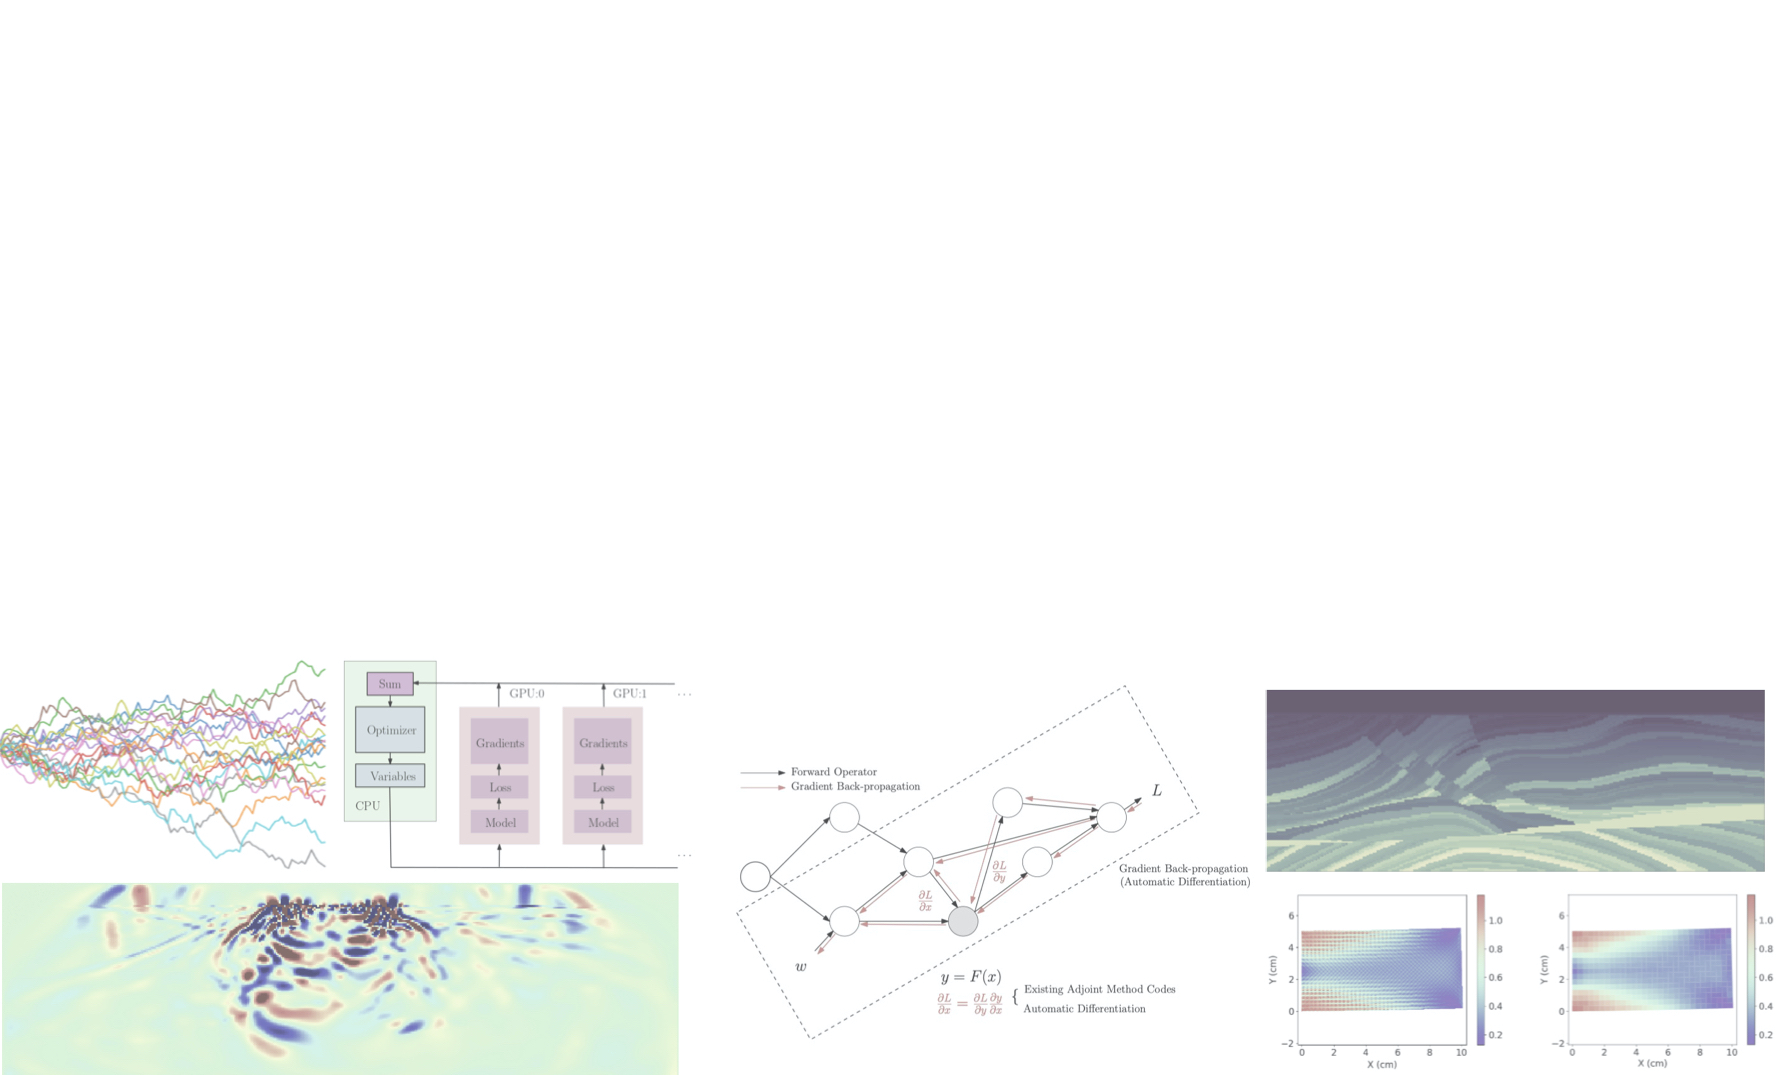
\includegraphics[width=1.0\paperwidth]{figures/background}}}
\end{picture}
  } 
%\usebackgroundtemplate{%
%  \includegraphics[width=\paperwidth,height=\paperheight]{figures/back}} 
\begin{frame}

\titlepage % Print the title page as the first slide

%dfa
\end{frame}
\usebackgroundtemplate{}

\section{Inverse Modeling}




\begin{frame}
	\frametitle{Inverse Modeling}
	\begin{figure}
	\centering
  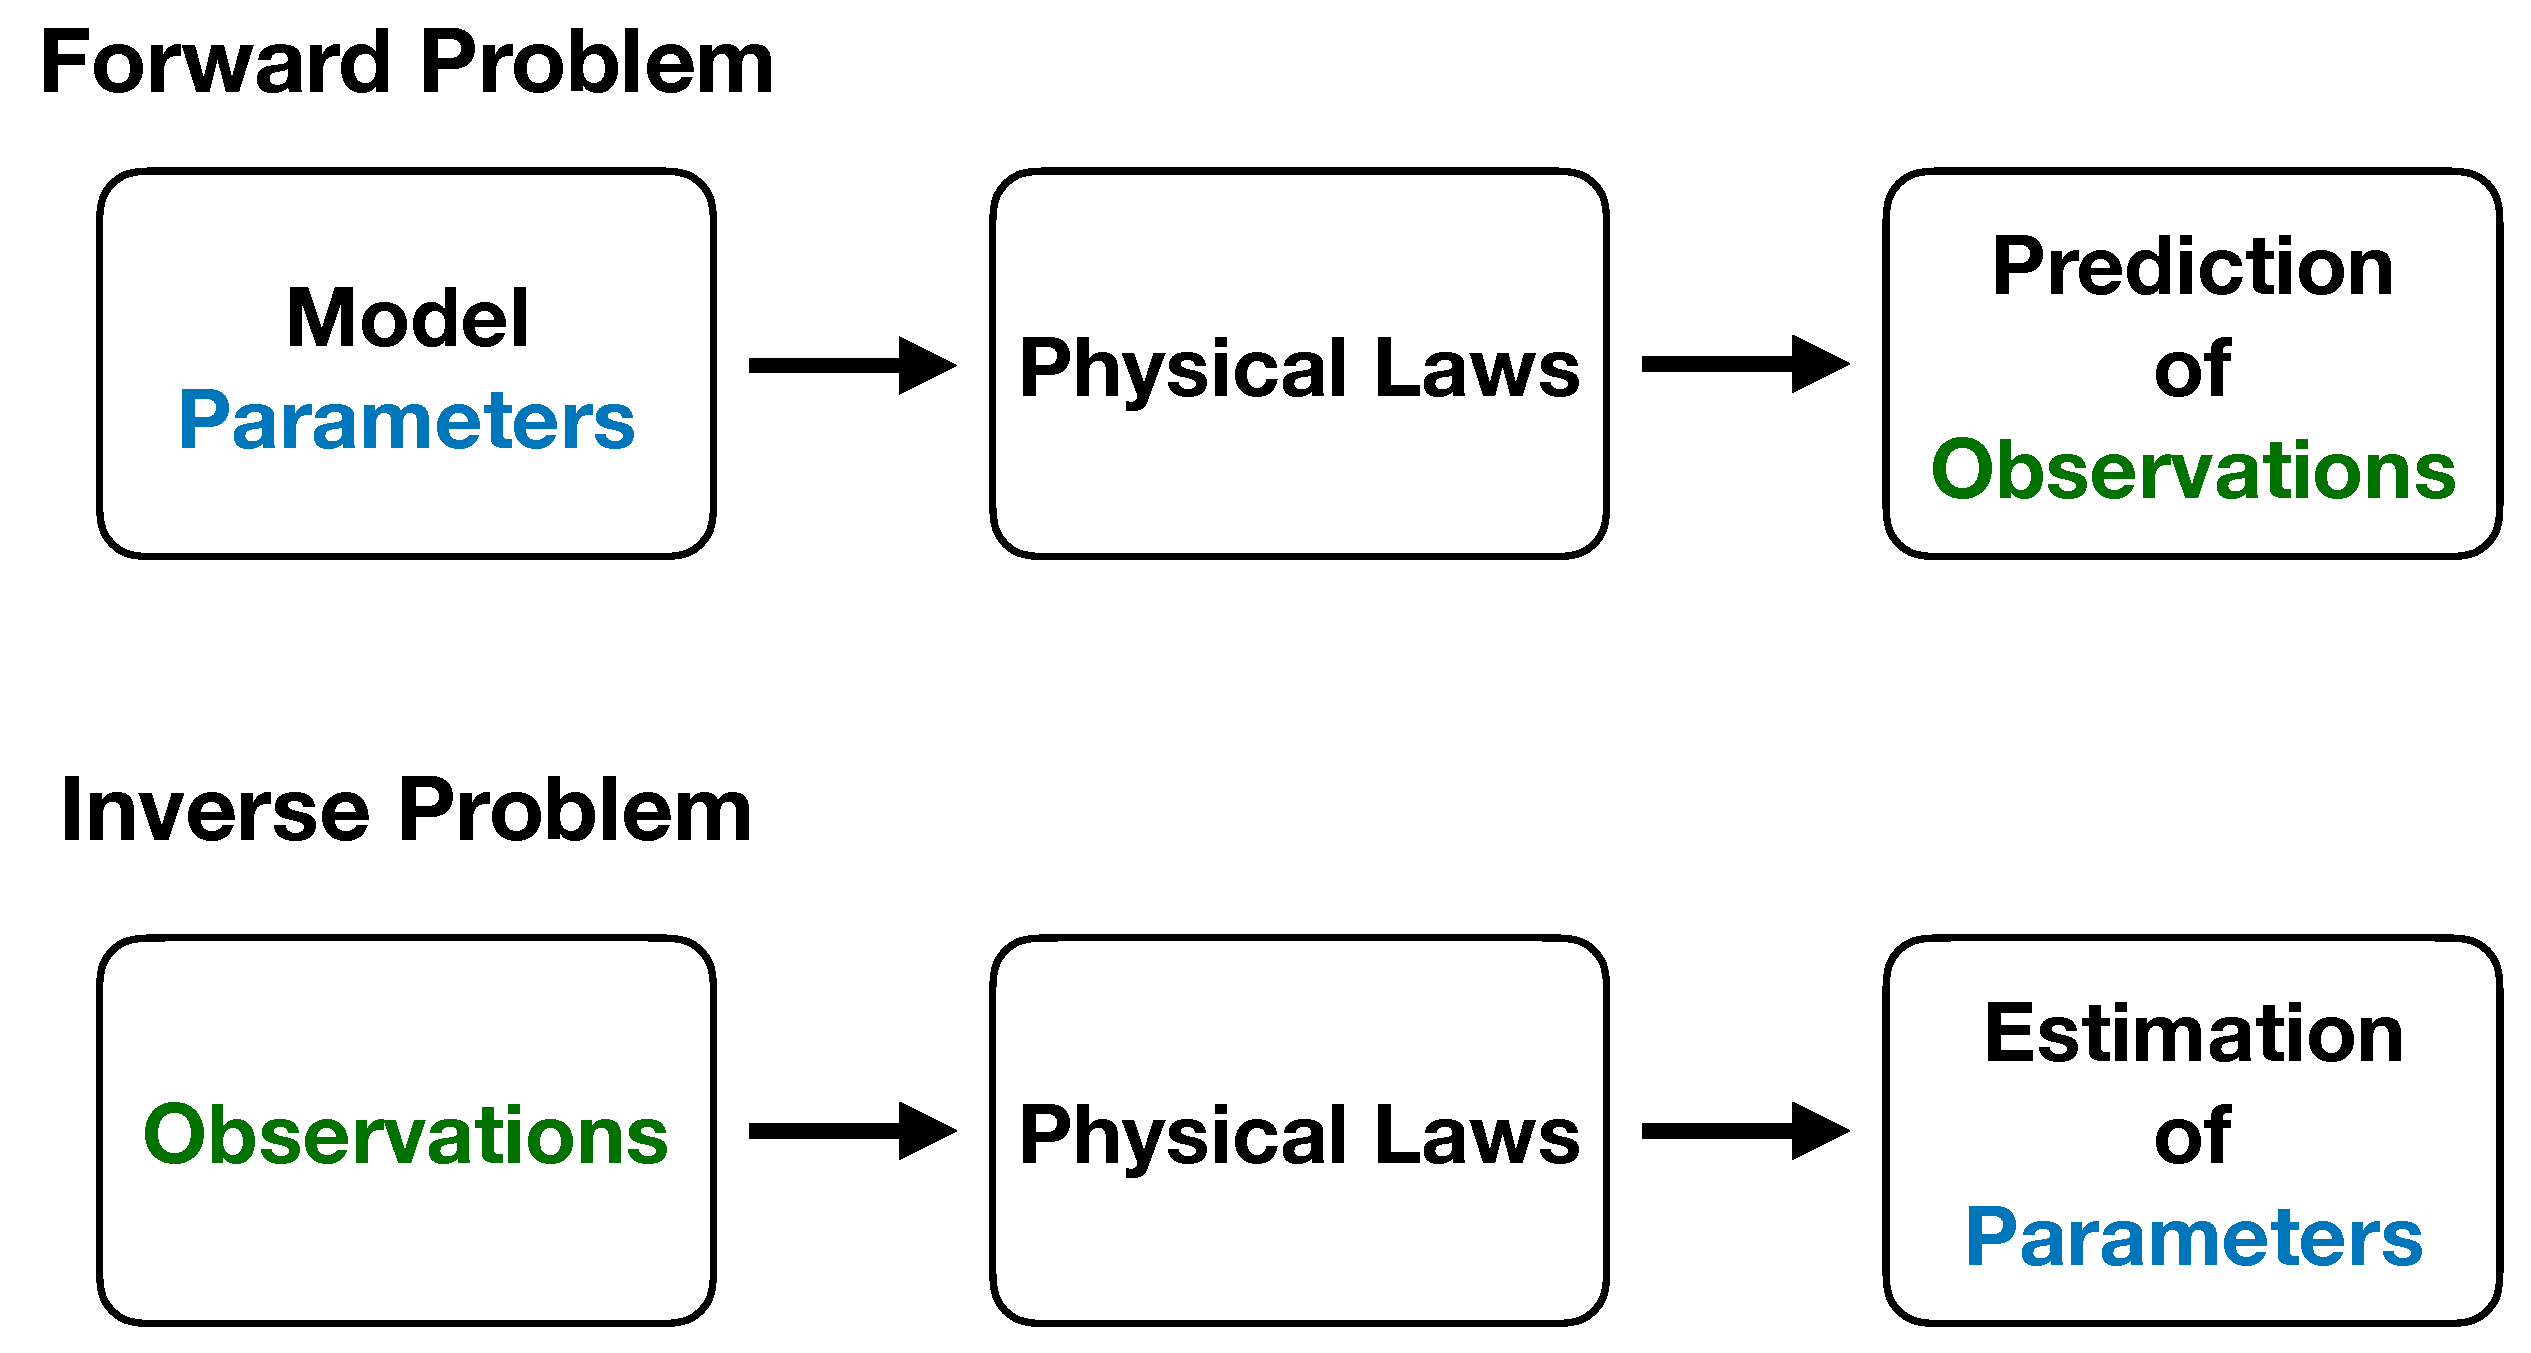
\includegraphics[width=1.0\textwidth]{figures/inverse3}
\end{figure}
\end{frame}

\begin{frame}
	\frametitle{Inverse Modeling}
	We can formulate inverse modeling as a PDE-constrained optimization problem 
	\begin{equation*}
		\min_{\theta} L_h(u_h) \quad \mathrm{s.t.}\; F_h(\theta, u_h) = 0
	\end{equation*}
	\begin{itemize}
		\item The \textcolor{red}{loss function} $L_h$ measures the discrepancy between the prediction $u_h$ and the observation $u_{\mathrm{obs}}$, e.g., $L_h(u_h) = \|u_h - u_{\mathrm{obs}}\|_2^2$. 
		\item $\theta$ is the \textcolor{red}{model parameter} to be calibrated. 
		\item The \textcolor{red}{physics constraints} $F_h(\theta, u_h)=0$ are described by a system of partial differential equations. Solving for $u_h$ may require solving linear systems or applying an iterative algorithm such as the Newton-Raphson method. 
	\end{itemize}
\end{frame}

\begin{frame}
	\frametitle{Function Inverse Problem}
	
	\begin{equation*}
		\min_{\textcolor{red}{f}} L_h(u_h) \quad \mathrm{s.t.}\; F_h(\textcolor{red}{f}, u_h) = 0
	\end{equation*}
	
	What if the unknown is a \textcolor{red}{function} instead of a set of parameters?
\begin{itemize}
	\item Koopman operator in dynamical systems.
	\item Constitutive relations in solid mechanics. 
	\item Turbulent closure relations in fluid mechanics.
	\item ...
\end{itemize}

The candidate solution space is \textcolor{red}{infinite dimensional}.

\end{frame}

\begin{frame}
	\frametitle{Machine Learning for Computational Engineering}
	$$\min_{\theta} L_h(u_h) \quad \mathrm{s.t.}\;F_h(\textcolor{red}{NN_\theta}, u_h) = 0$$
	\vspace{-0.5cm}
	\begin{itemize}
		\item Deep neural networks exhibit capability of approximating high dimensional and complicated functions. 
		\item \textbf{Machine Learning for Computational Engineering}: \textcolor{red}{the unknown function is approximated by a deep neural network, and the physical constraints are enforced by numerical schemes}.
		\item \textcolor{red}{Satisfy the physics to the largest extent}.
	\end{itemize}
	\begin{figure}[hbt]
  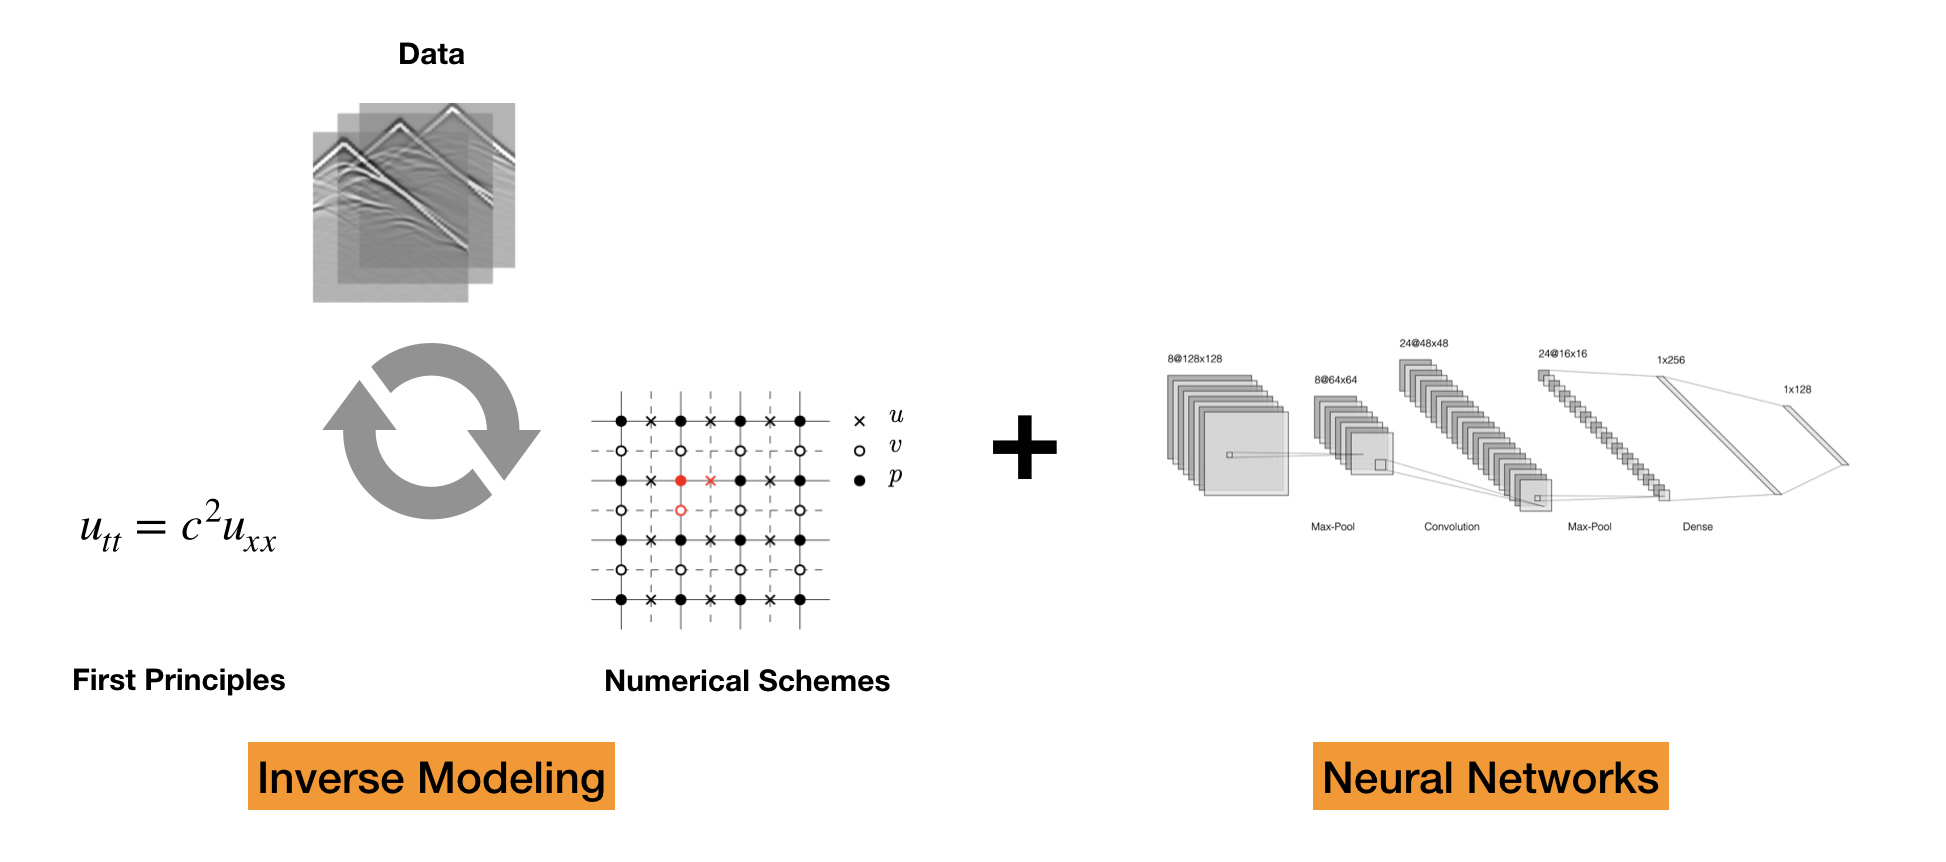
\includegraphics[width=0.75\textwidth]{figures/physics_based_machine_learning.png}
\end{figure}
\end{frame}



\begin{frame}
	\frametitle{Gradient Based Optimization}
	\begin{equation}\label{equ:opt}
		\min_{\theta} L_h(u_h) \quad \mathrm{s.t.}\; F_h(\theta, u_h) = 0
		\end{equation}
	
	\begin{itemize}
		\item We can now apply a gradient-based optimization method to (\ref{equ:opt}).
		\item The key is to \textcolor{red}{calculate the gradient descent direction} $g^k$
		$$\theta^{k+1} \gets \theta^k - \alpha g^k$$ 
	\end{itemize}
	
	\begin{figure}[hbt]
	\centering
  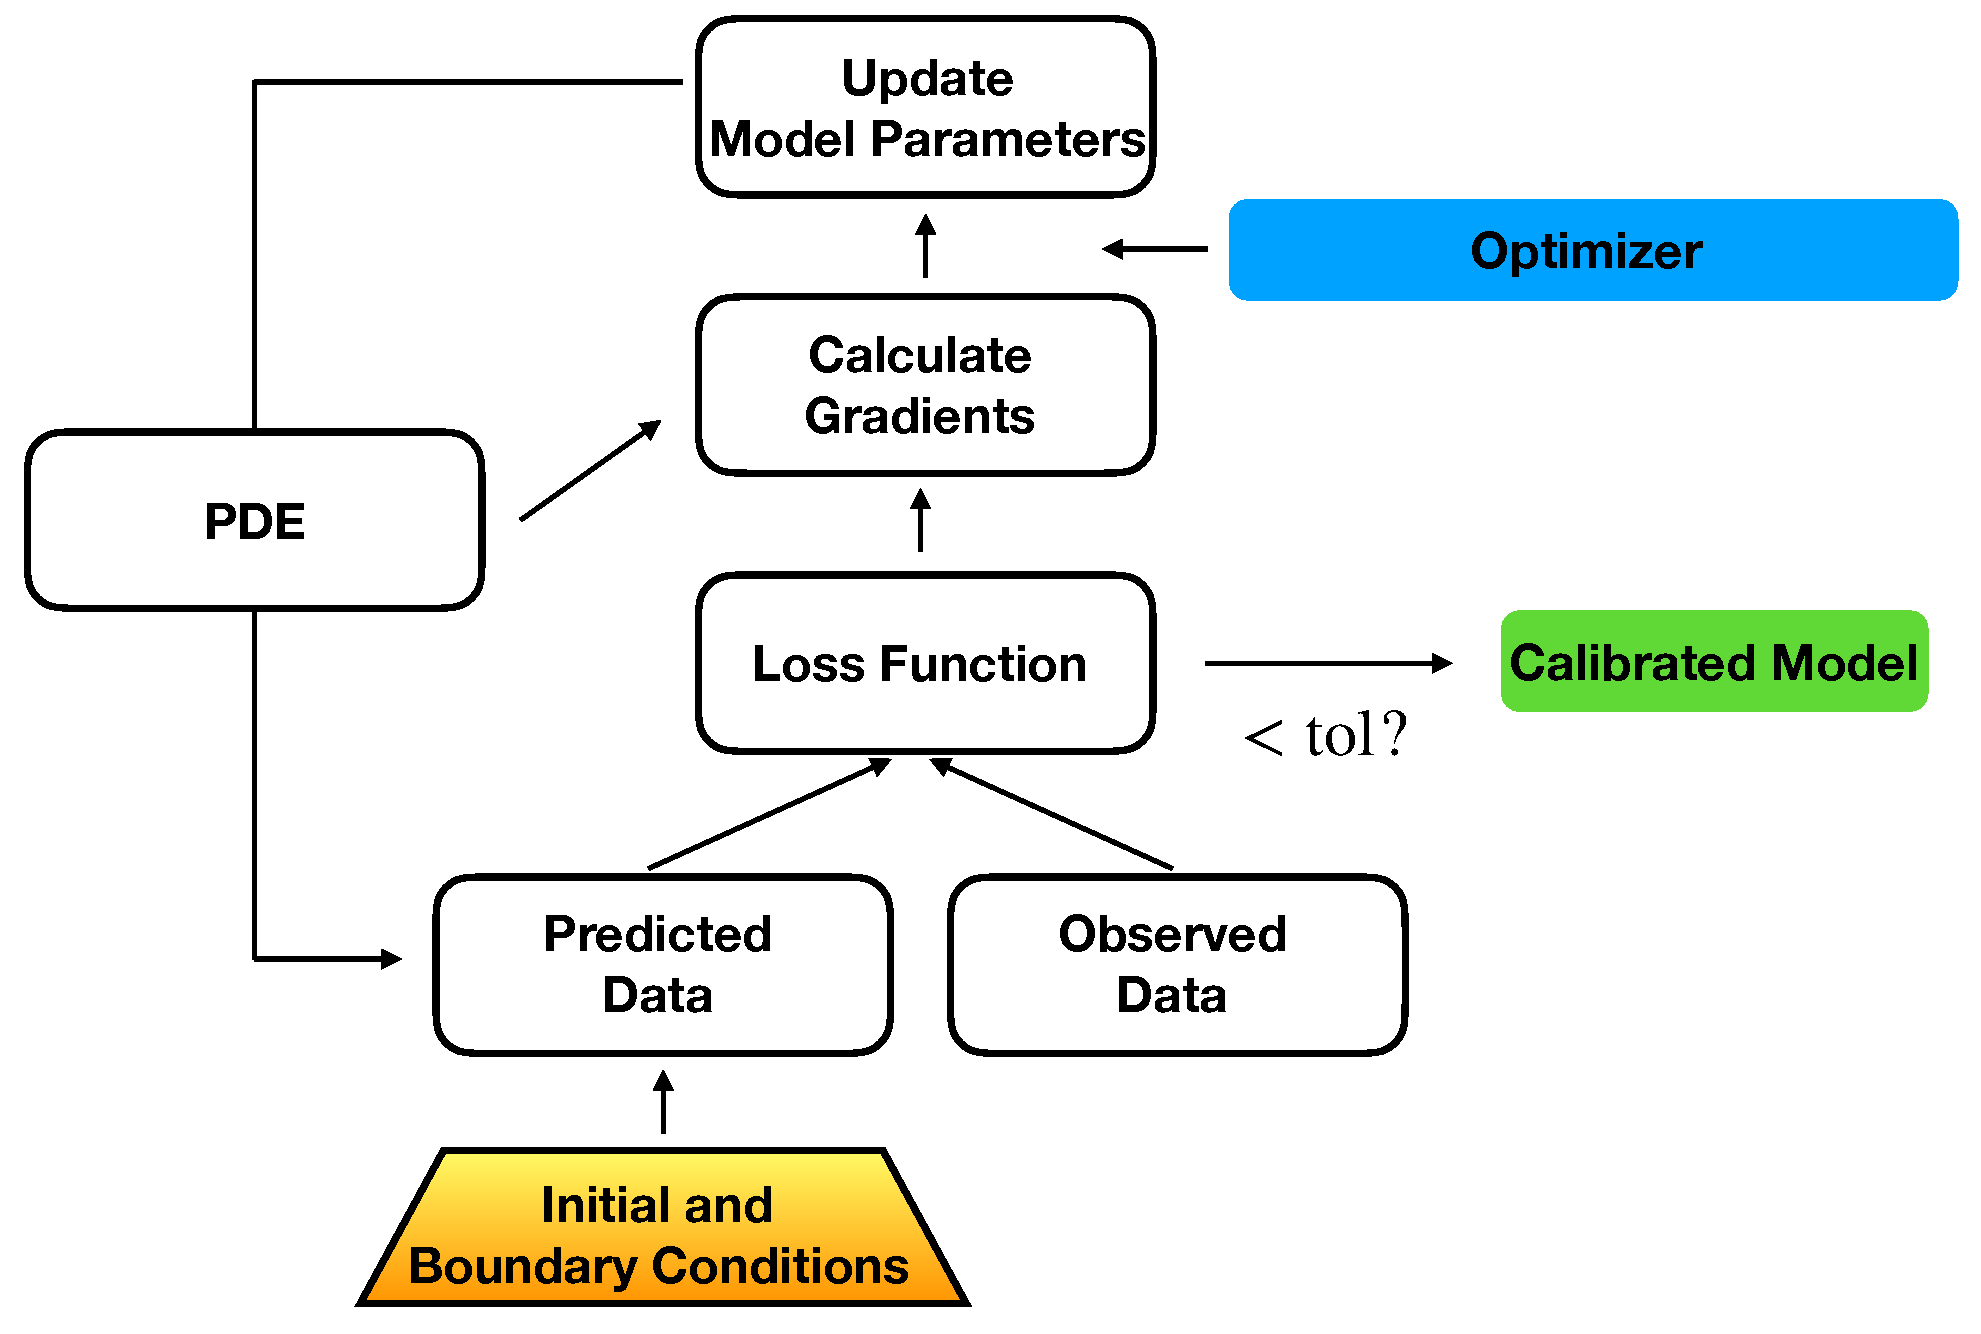
\includegraphics[width=0.6\textwidth]{figures/im.pdf}
\end{figure}

\end{frame}



\section{Automatic Differentiation}


\begin{frame}
	\frametitle{Automatic Differentiation}
	The fact that bridges the \textcolor{red}{technical} gap between machine learning and inverse modeling:
	\begin{itemize}
		\item Deep learning (and many other machine learning techniques) and numerical schemes share the same computational model: composition of individual operators. 
	\end{itemize}
	
	
	\begin{minipage}[t]{0.4\textwidth}
		
		\
		
		
		
		\begin{center}
			\textcolor{red}{Mathematical Fact}
			
			\
			
			Back-propagation 
			
			$||$
			
			Reverse-mode
			
			Automatic Differentiation 
			
			$||$
			
			Discrete 
			
			Adjoint-State Method
		\end{center}
	\end{minipage}~
	\begin{minipage}[t]{0.6\textwidth}
		\begin{figure}[hbt]
			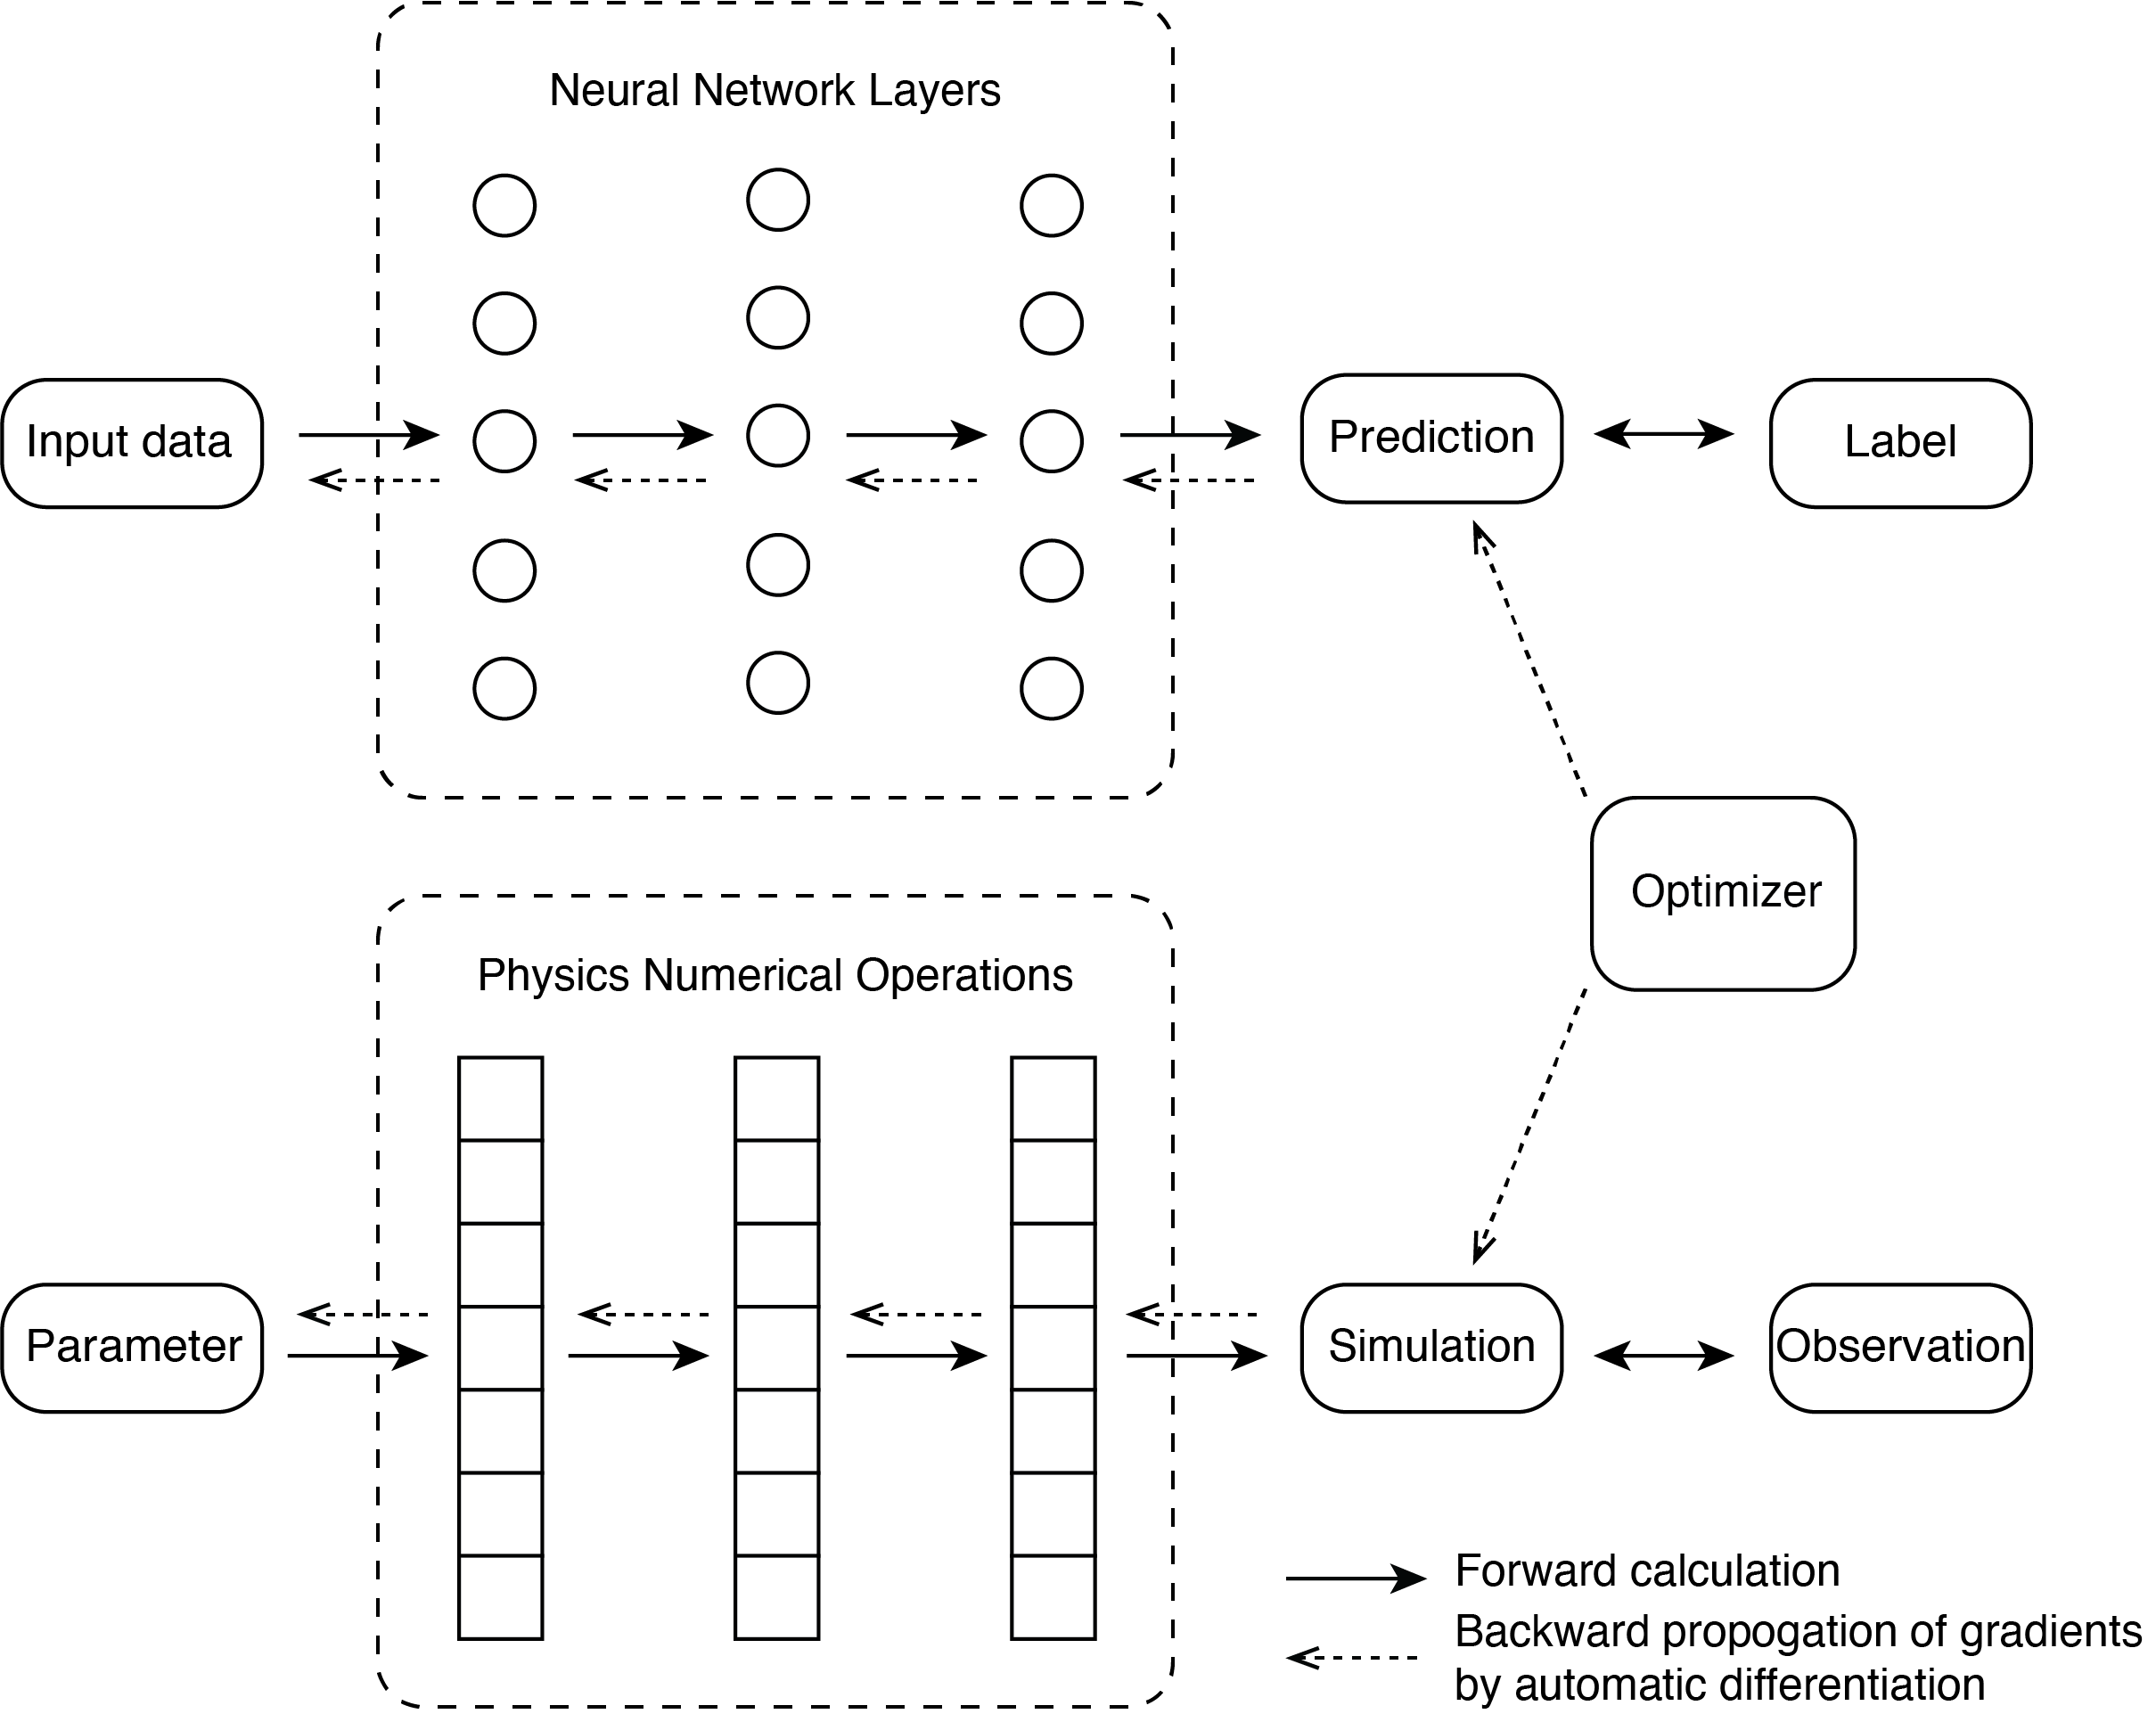
\includegraphics[width=0.8\textwidth]{figures/compare-NN-PDE.png}
		\end{figure}
	\end{minipage}
	
\end{frame}

\begin{frame}
	\frametitle{Computational Graph for Numerical Schemes}
	
	\begin{itemize}
		\item To leverage automatic differentiation for inverse modeling, we need to express the numerical schemes in the ``AD language'': computational graph. 
		\item No matter how complicated a numerical scheme is, it can be decomposed into a collection of operators that are interlinked via state variable dependencies. 
	\end{itemize}
	
	\begin{figure}[hbt]
		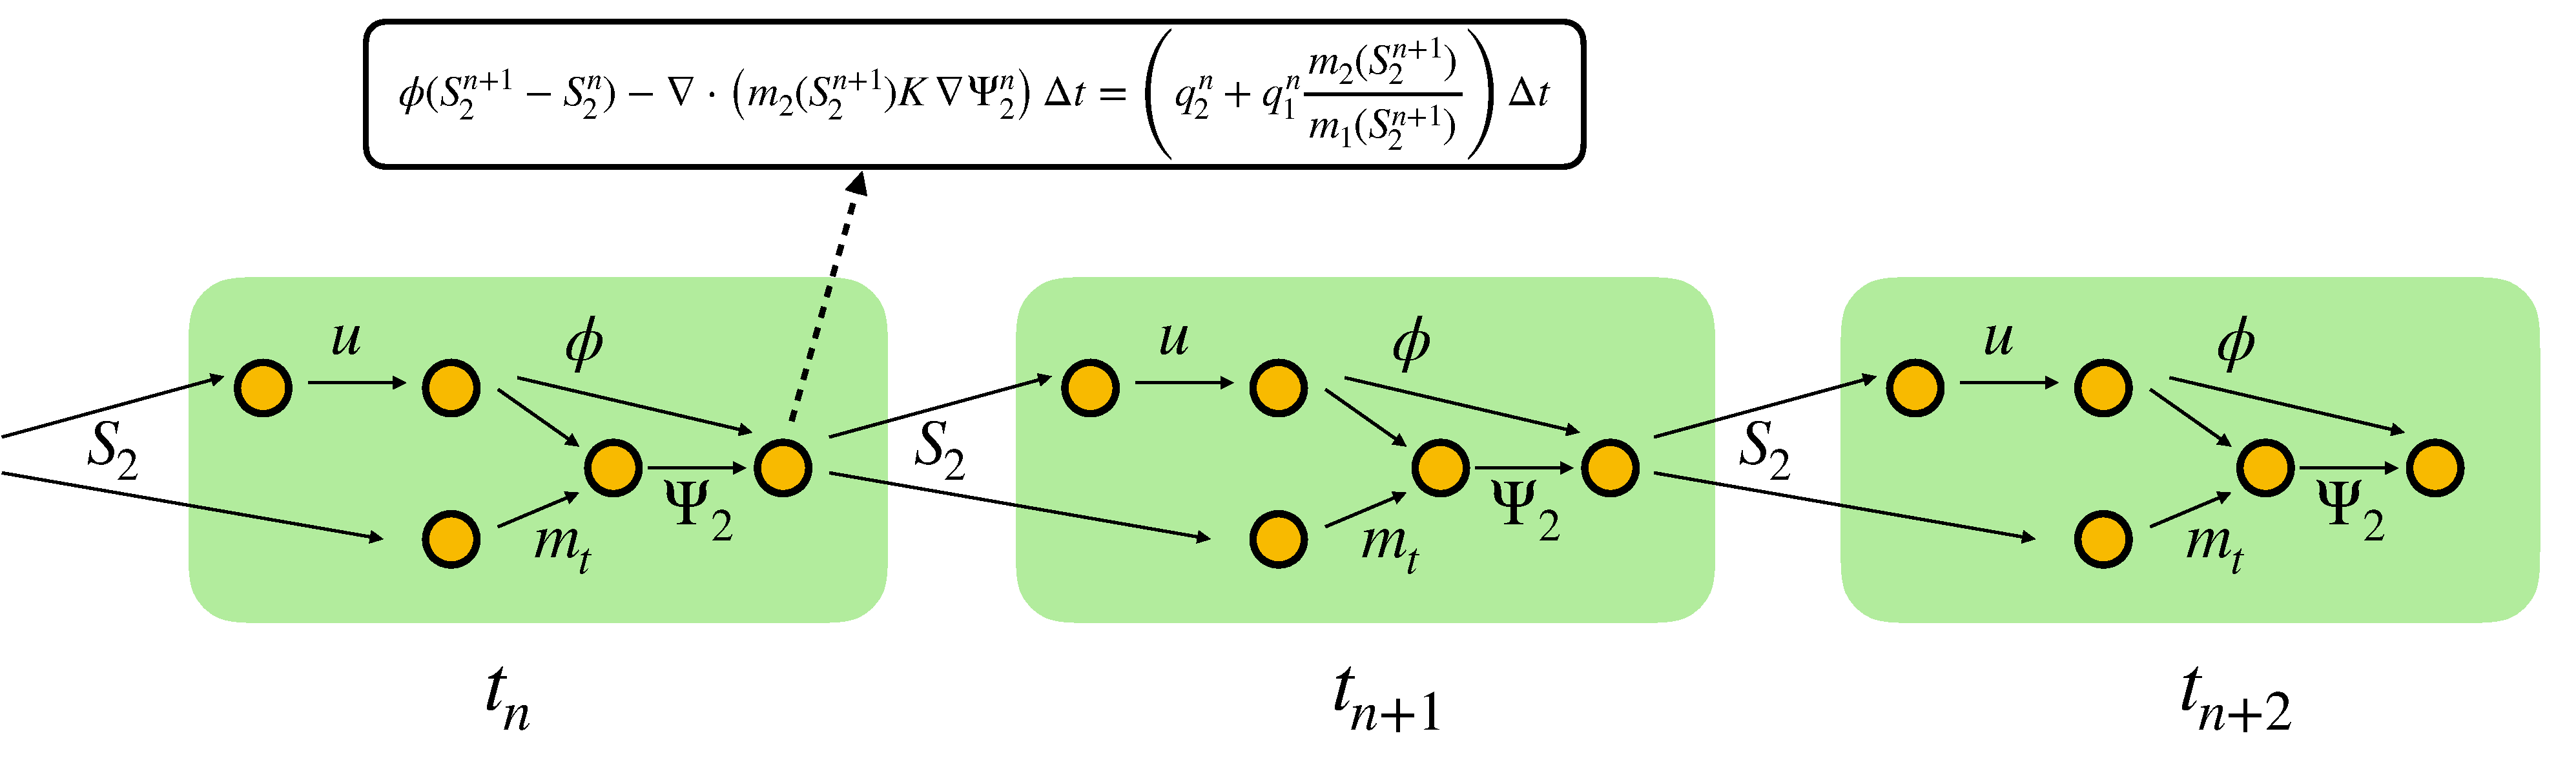
\includegraphics[width=1.0\textwidth]{figures/cgnum}
	\end{figure}
	
	
	
\end{frame}


\begin{frame}
	\frametitle{ADCME: Computational-Graph-based Numerical Simulation}
	
	\begin{figure}[hbt]
		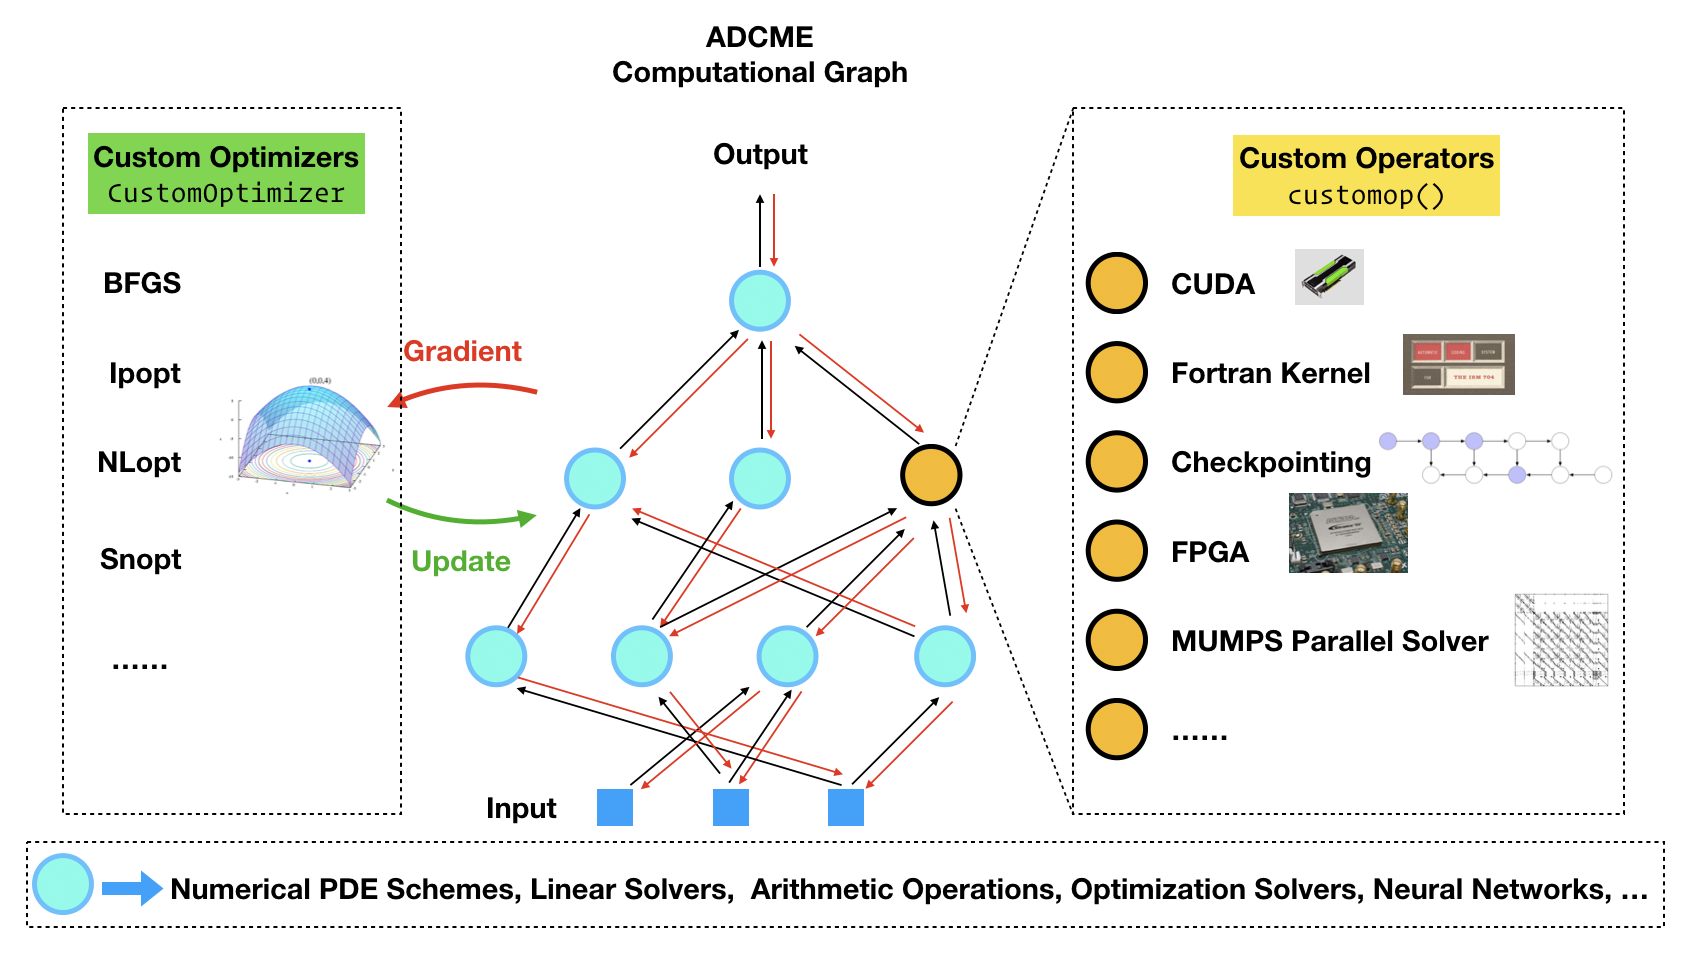
\includegraphics[width=1.0\textwidth]{figures/custom}
	\end{figure}
\end{frame}


\begin{frame}
	\frametitle{Automatic Differentiation: Forward-mode and Reverse-mode}
	\begin{figure}
		\centering
		\includegraphics[width=1.0\textwidth]{figures/forwardreverse}
	\end{figure}
\end{frame}


\begin{frame}
	\frametitle{What is the Appropriate Model for Inverse Problems?}
	
	\begin{itemize}
		\item In general, for a function $f:\RR^n \rightarrow \RR^m$
		% Please add the following required packages to your document preamble:
		% \usepackage{booktabs}
		\begin{table}[]
			\centering
			\begin{tabular}{@{}llll@{}}
				\toprule
				Mode & Suitable for ... & Complexity\footnote{$\mathrm{OPS}$ is a metric for complexity in terms of fused-multiply adds.} & Application \\ \midrule
				Forward & $m\gg n$ & $\leq 2.5\;\mathrm{OPS}(f(x))$ & UQ \\
				Reverse & $m\ll n$ & $\leq 4\;\mathrm{OPS}(f(x))$ & Inverse Modeling \\ \bottomrule
			\end{tabular}
		\end{table}
		
		
		\item There are also many other interesting topics
		\begin{itemize}
			\item Mixed mode AD: many-to-many mappings.
			\item Computing sparse Jacobian matrices using AD by exploiting sparse structures. 
		\end{itemize}
	\end{itemize}
	{\scriptsize Margossian CC. A review of automatic differentiation and its efficient implementation. Wiley Interdisciplinary Reviews: Data Mining and Knowledge Discovery. 2019 Jul;9(4):e1305.} 
\end{frame}






\begin{frame}
	\frametitle{Granularity of Automatic Differentiation}
	
	
	\begin{figure}[hbt]
		\centering
		\includegraphics[width=0.8\textwidth]{figures/adlevel}
	\end{figure}
	
	
	
\end{frame}


\section{Code Example}


\begin{frame}
	\frametitle{Inverse Modeling of the Stokes Equation}
	
	\begin{itemize}
		\item The governing equation for the Stokes problem
			$$\begin{aligned} -\textcolor{red}{\nu}\Delta \mathbf{u} + \nabla p &= \mathbf{f} & \text{ in } \Omega \\ \nabla \cdot \mathbf{u} &= 0 & \text{ in } \Omega \\ \mathbf{u} &= \mathbf{0} & \text{ on } \partial \Omega \end{aligned}$$
	\end{itemize}


\begin{minipage}[c]{0.7\textwidth}
\begin{itemize}
	\item The weak form is given by 
	\begin{equation*}
		\begin{aligned}
			(\textcolor{red}{\nu} \nabla u, \nabla v) &- (p, \nabla \cdot v) &&= (f, v)\\
			(\nabla \cdot u, q) & &&= 0
		\end{aligned}
	\end{equation*}
\end{itemize}
\end{minipage}~
\begin{minipage}[c]{0.29\textwidth}
	\includegraphics[width=1.0\textwidth]{figures/stokesuvp}
\end{minipage}


\end{frame}


\begin{frame}[fragile]{}
	\frametitle{Inverse Modeling of the Stokes Equation}
	
	\begin{minted}[escapeinside=||,fontsize=\small]{julia}
|\textbf{\colorbox{green}{nu = \texttt{Variable(0.5)}}}|
K = nu*constant(|\underline{\texttt{compute\_fem\_laplace\_matrix}}|(m, n, h))
B = constant(|\underline{\texttt{compute\_interaction\_matrix}}|(m, n, h))
Z = [K -B'
    -B spdiag(zeros(size(B,1)))]

# Impose boundary conditions
bd = bcnode("all", m, n, h)
bd = [bd; bd .+ (m+1)*(n+1); ((1:m) .+ 2(m+1)*(n+1))]
Z, _ = |\underline{\texttt{fem\_impose\_Dirichlet\_boundary\_condition1}}|(Z, bd, m, n, h)

# Calculate the source term 
F1 = |\underline{\texttt{eval\_f\_on\_gauss\_pts}}|(f1func, m, n, h)
F2 = |\underline{\texttt{eval\_f\_on\_gauss\_pts}}|(f2func, m, n, h)
F = |\underline{\texttt{compute\_fem\_source\_term}}|(F1, F2, m, n, h)
rhs = [F;zeros(m*n)]
rhs[bd] .= 0.0

sol = Z\rhs 
	\end{minted}
	
	
\end{frame}



\begin{frame}[fragile]{}
	\frametitle{Inverse Modeling of the Stokes Equation}
	
	\begin{itemize}
		\item The distinguished feature compared to traditional forward simulation programs: \textcolor{red}{the model output is differentiable with respect to model parameters}!
		\begin{minted}[escapeinside=||,fontsize=\small]{julia}
loss = sum((sol[idx] - observation[idx])^2)
g = gradients(loss, nu)
		\end{minted}
		\item Optimization with a one-liner:
\begin{minted}[escapeinside=||,fontsize=\small]{julia}
BFGS!(sess, loss)
\end{minted}	 
	\end{itemize}

	\begin{figure}[hbt]
	\centering
	\includegraphics[width=0.8\textwidth]{figures/lego}
\end{figure}
	
\end{frame}


%\begin{frame}
%	\frametitle{Code Example}
%	\begin{itemize}
%		\item  Find $b$ such that $u(0.5)=1.0$ and
%		$$-bu''(x)+u(x) = 8 + 4x - 4x^2, x\in[0,1], u(0)=u(1)=0$$
%	\end{itemize}
%	\begin{figure}[hbt]
%  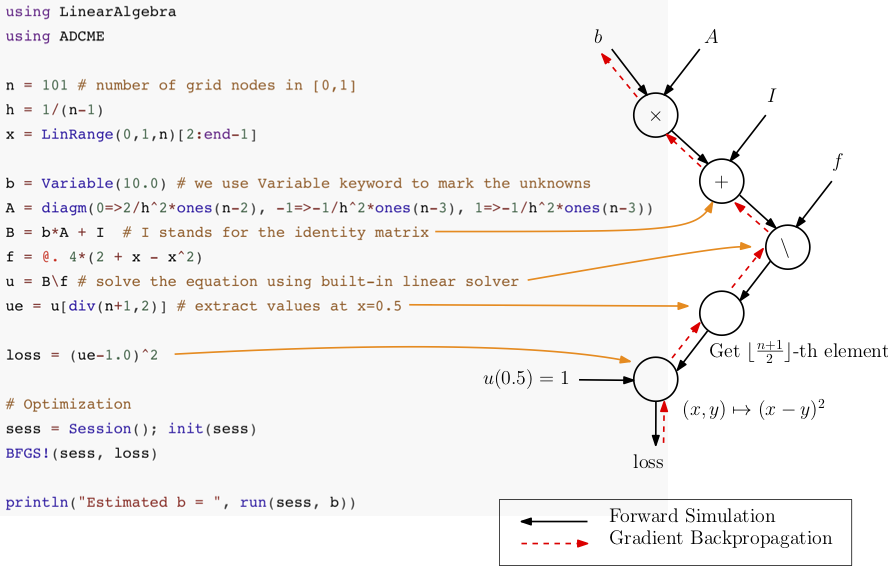
\includegraphics[width=0.8\textwidth]{figures/code.png}
%\end{figure}
%\end{frame}




\section{Applications}


\newcommand{\bsigma}[0]{\bm{\sigma}}
\newcommand{\bepsilon}[0]{\bm{\epsilon}}


\begin{frame}
	
	\frametitle{Linear Poroelasticity}
	
	\begin{itemize}
		\item The governing equation for linear poroelasticity with a spatially-varying viscosity coefficient 
		\begin{equation*}
				\begin{aligned}
					\text{div} \bsigma + \rho \mathbf{g} &=  \ddot \bu \\ 
					\dot \sigma_{ij} + \frac{\mu}{\textcolor{red}{\eta(y)}} \left( \sigma_{ij} - \frac{\sigma_{kk}}{3} \delta_{ij} \right) &= 2\mu \dot \epsilon_{ij} + \lambda \dot \epsilon_{kk} \delta_{ij}
				\end{aligned}
		\end{equation*}
		
		\begin{figure}
			\centering
			\includegraphics[width=0.5\textwidth]{figures/poroelasticity_bc.png}
		\end{figure}
	\end{itemize}
	
\end{frame}




\begin{frame}
	
	\frametitle{Linear Poroelasticity}
	
	\begin{itemize}
		\item The true model of $\eta(y)^{-1}$, the displacement at the terminal time, and the von Mises 
		stress distribution at the terminal time. 
		\begin{figure}
			\centering
			\includegraphics[width=0.8\textwidth]{figures/poroelasticity_1.png}
		\end{figure}
	
		\item Evolution of learned $\eta(y)^{-1}$ at iteration 0, 80, 160, and 240. 
		\begin{figure}
			\centering
			\includegraphics[width=0.8\textwidth]{figures/poroelasticity_2.png}
		\end{figure}
	\end{itemize}
	
\end{frame}


\begin{frame}

	\frametitle{Viscoelasticity}
	%	
	\begin{itemize}
		\item Multi-physics Interaction of Coupled Geomechanics and Multi-Phase Flow Equations 
		{\small
			\begin{align*}
			\mathrm{div}\bsigma(\bu) - b \nabla p &= 0\\
			\frac{1}{M} \frac{\partial p}{\partial t} + b\frac{\partial \epsilon_v(\bu)}{\partial t} - \nabla\cdot\left(\frac{k}{B_f\mu}\nabla p\right) &= f(x,t)	\\
			\bsigma &= \bsigma(\bepsilon, \dot\bepsilon)
			\end{align*}
		}
		\item Approximate the constitutive relation by a neural network
		{\small
			$$\bsigma^{n+1} = \mathcal{NN}_{\bt} (\bsigma^n, \bepsilon^n) + H\bepsilon^{n+1}$$}
	\end{itemize}		
	\begin{figure}[hbt]	
		\centering
		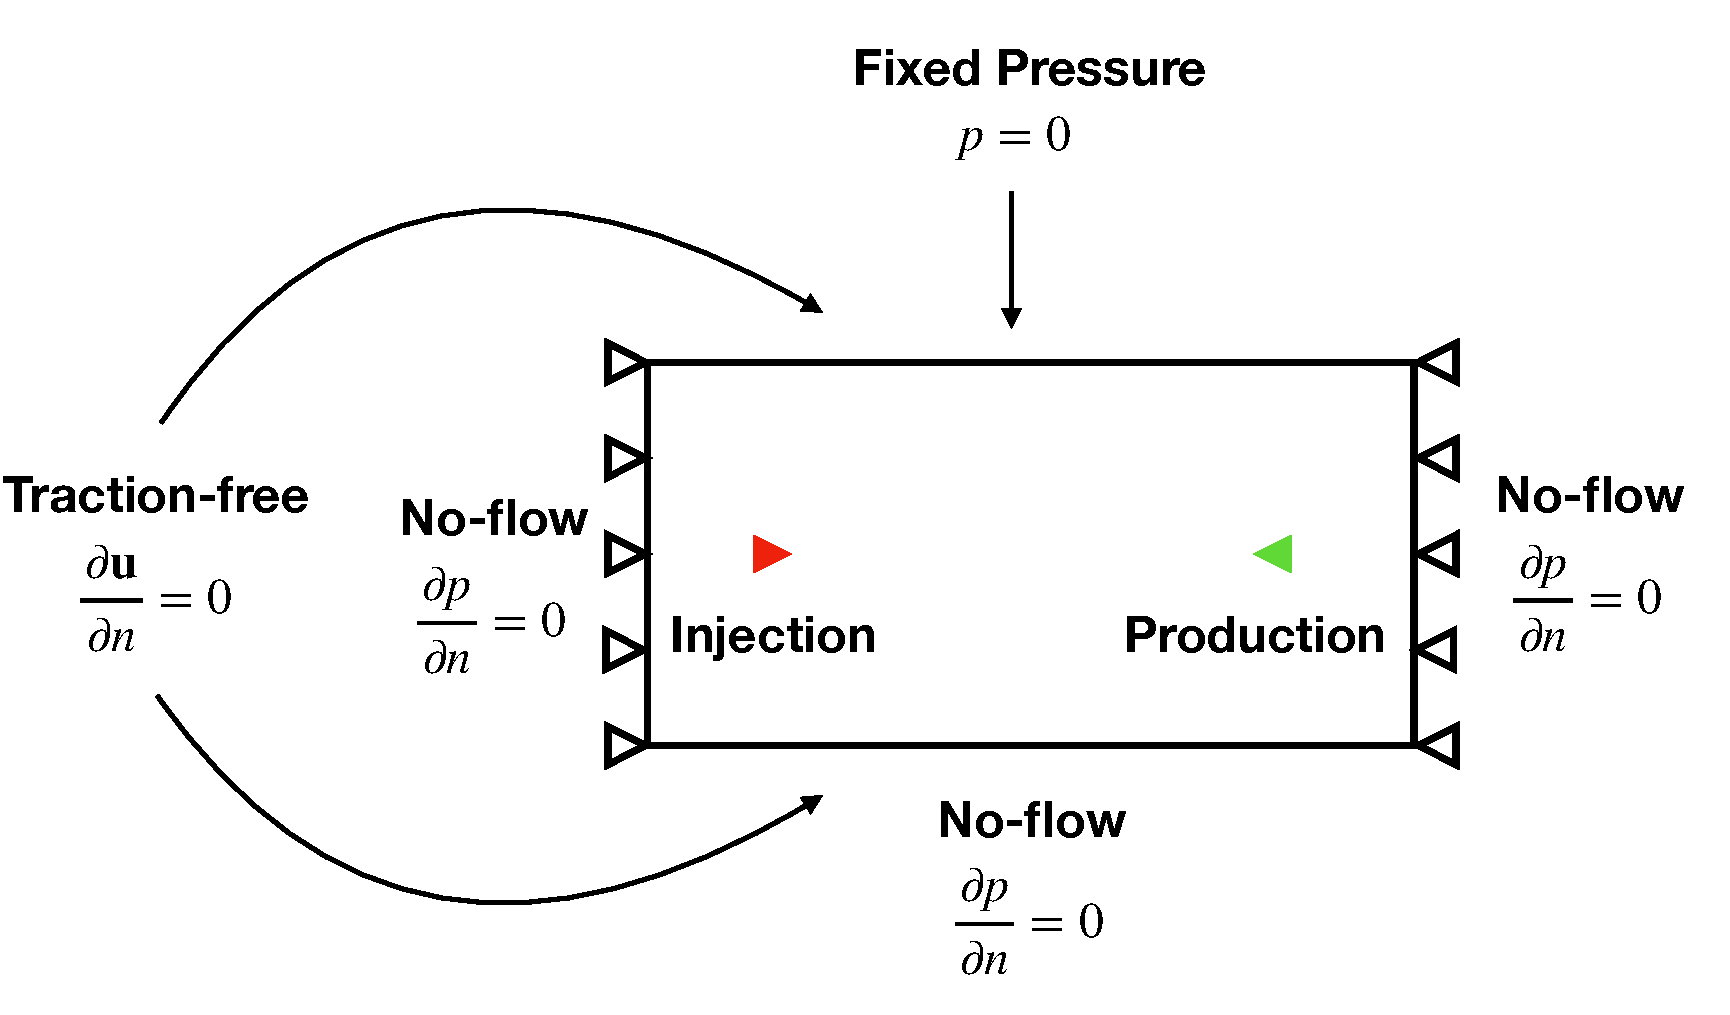
\includegraphics[width=0.5\textwidth]{../ip}~
		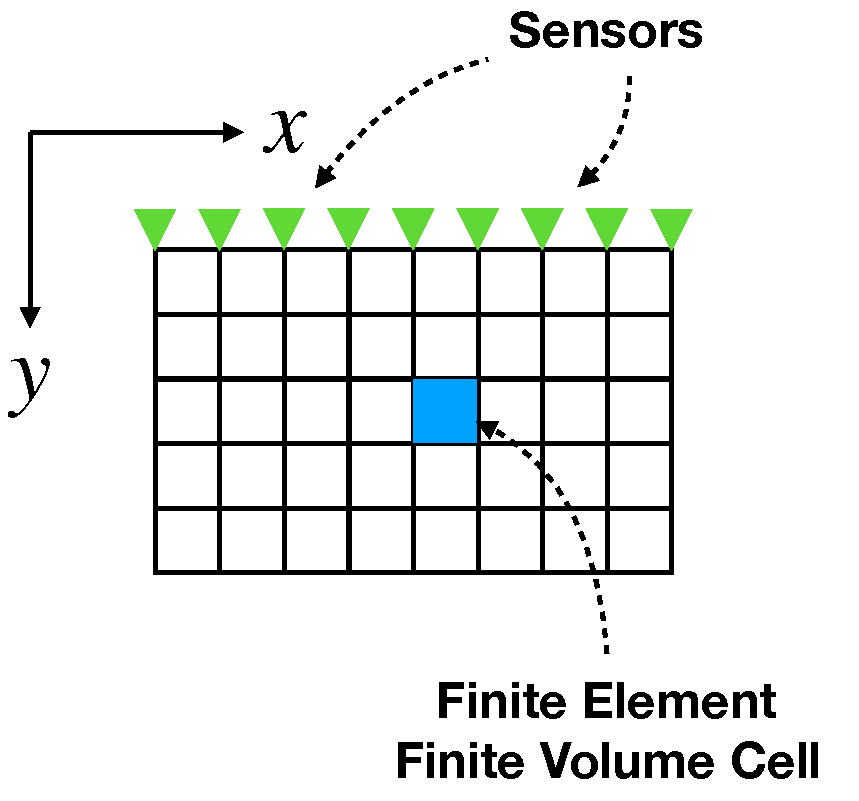
\includegraphics[width=0.3\textwidth]{../cell}
	\end{figure}
	
\end{frame}


\begin{frame}
	\frametitle{Viscoelasticity}
	
	\begin{itemize}
		\item Comparison with space varying linear elasticity approximation
		\begin{equation*}
		\bsigma = H(x, y) \bepsilon
		\end{equation*}
	\end{itemize}
	\begin{figure}[hbt]
		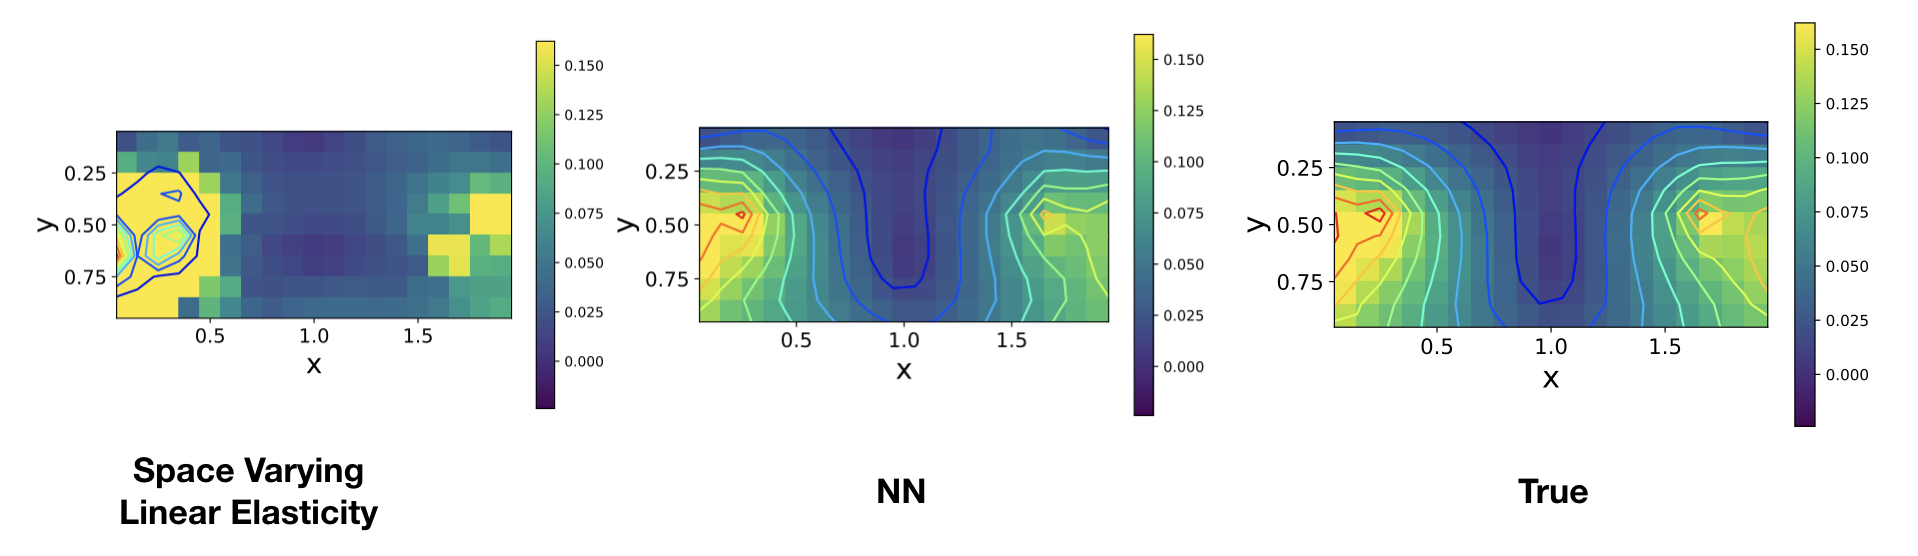
\includegraphics[width=1.0\textwidth]{../visco1}
	\end{figure}
	
\end{frame}

\begin{frame}
	\frametitle{Viscoelasticity}
	\begin{figure}[hbt]
		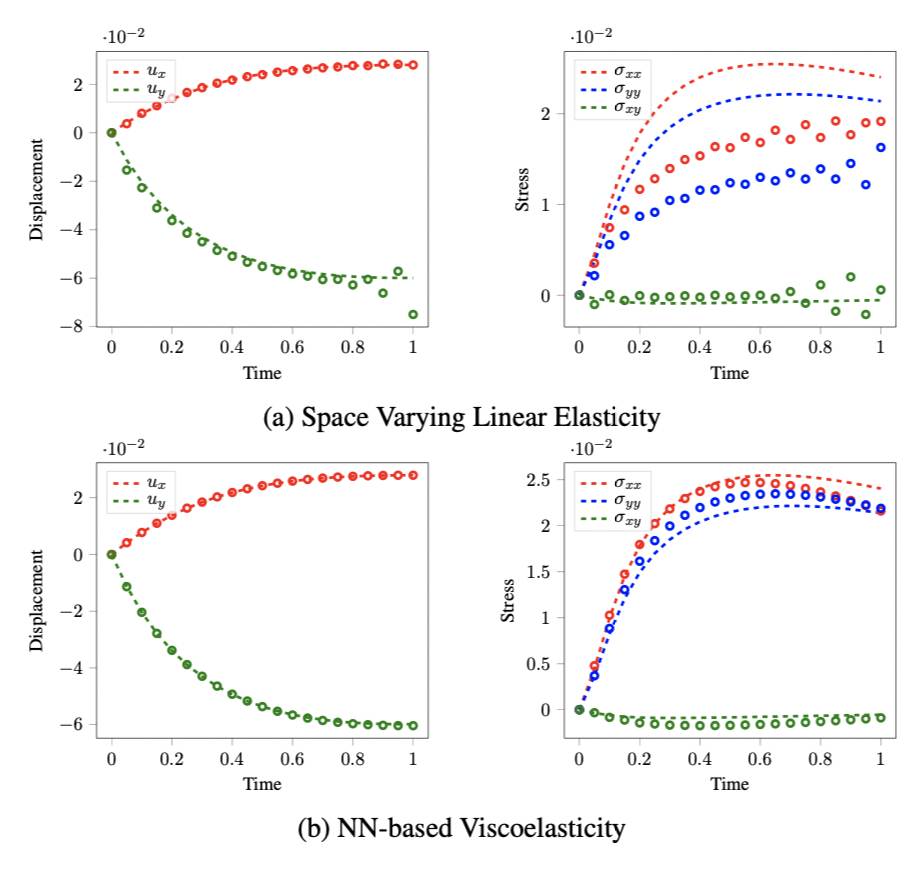
\includegraphics[width=0.7\textwidth]{../visco2}
	\end{figure}
	
\end{frame}


\begin{frame}
	\frametitle{Navier-Stokes Equation}
	\begin{itemize}
		\item Steady-state Navier-Stokes equation
		\begin{equation*}
		\begin{aligned}
		(\mathbf{u} \cdot \nabla) \mathbf{u} &=
		-\frac{1}{\rho} \nabla p + \nabla\cdot (\textcolor{red}{\nu} \nabla \mathbf{u}) + \mathbf{g}\\
		\nabla \cdot \mathbf{u} &= 0
		\end{aligned}
		\end{equation*}
		
		\item Inverse problem are ubiquitous in fluid dynamics:
		
		\begin{figure}[hbt]
			\centering
			\includegraphics[width=0.4\textwidth]{figures/icepack}~
			\includegraphics[width=0.4\textwidth]{figures/covid}
			\caption{Left: electronic cooling; right: nasal drug delivery.}
		\end{figure}
		
	\end{itemize}
	
\end{frame}


\begin{frame}
	\frametitle{Navier-Stokes Equation}
	
	\begin{figure}[hbt]
		\centering
		\includegraphics[width=0.49\textwidth]{figures/advertisement}~
		\includegraphics[width=0.49\textwidth]{figures/computational_graph}
	\end{figure}
\end{frame}



\begin{frame}
	\frametitle{Navier-Stokes Equation}
	\begin{itemize}
		\item Data: $(u, v)$
		\item Unknown: $\nu(\mathbf{x})$ (represented by a deep neural network)
		\item Prediction: $p$ (absent in the training data) 
		\item The DNN provides regularization, which generalizes the estimation better!
	\end{itemize}
	\begin{figure}[hbt]
		\centering
		\includegraphics[width=1.0\textwidth]{figures/ns_result}~
	\end{figure}
\end{frame}

\begin{frame}
	\frametitle{A General Approach to Inverse Modeling}
	\begin{figure}[hbt]
		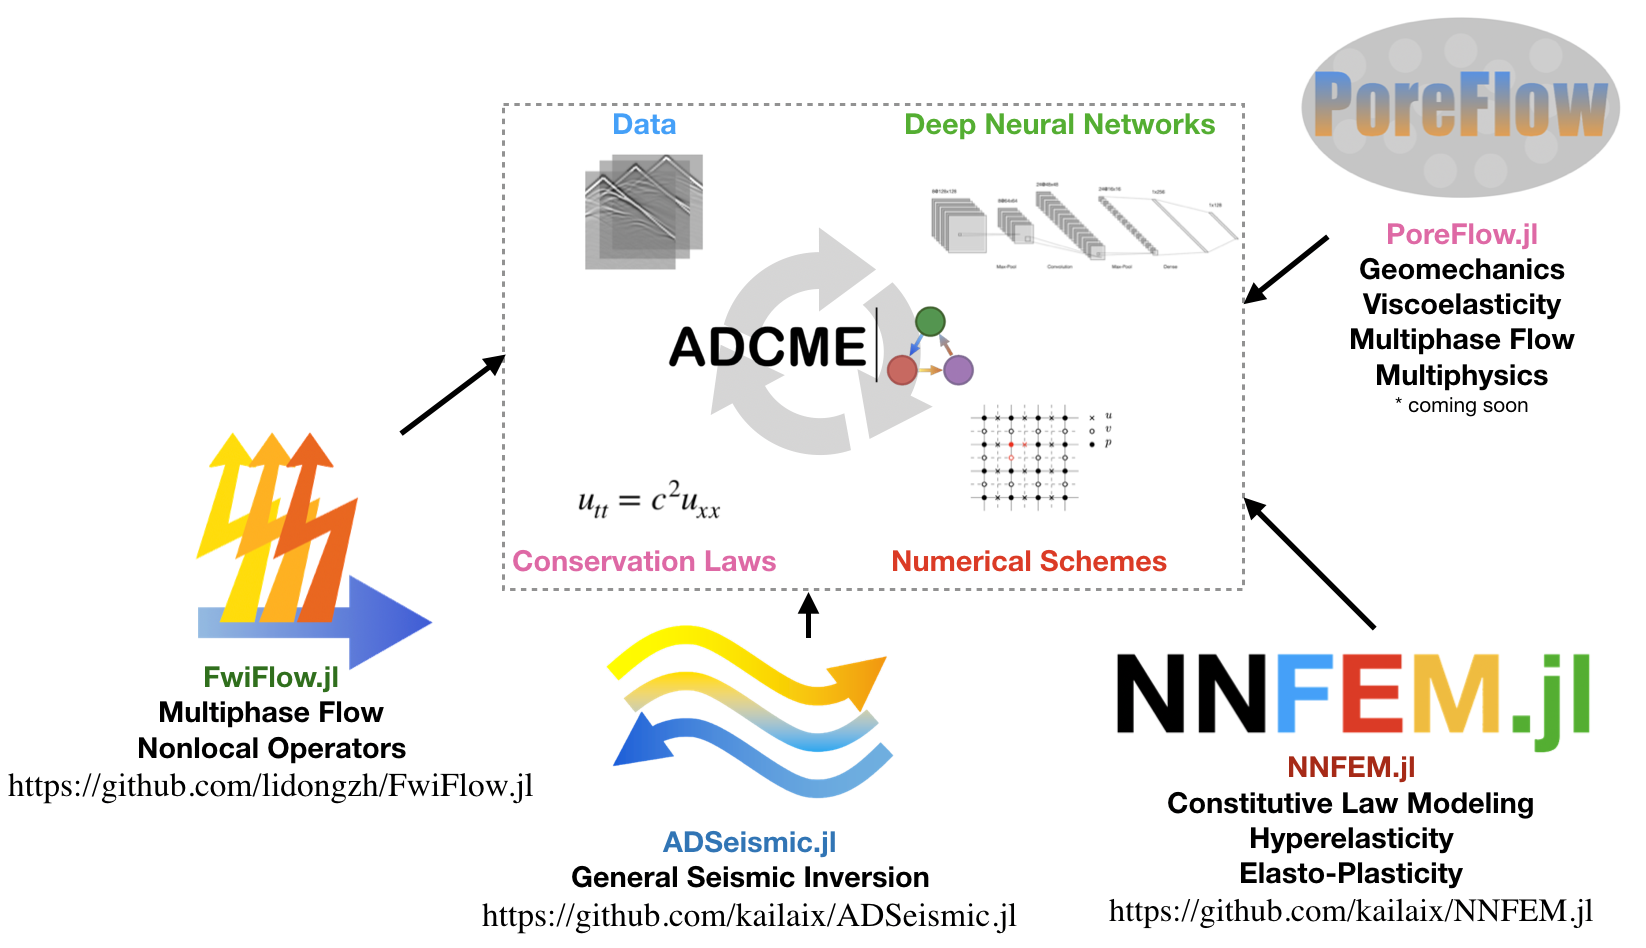
\includegraphics[width=1.0\textwidth]{figures/summary.png}
	\end{figure}
\end{frame}


%}
%\usebackgroundtemplate{}
%----------------------------------------------------------------------------------------
%    PRESENTATION SLIDES
%----------------------------------------------------------------------------------------

%------------------------------------------------



\end{document} 